\documentclass[11pt,a4paper]{article}

\usepackage[a4paper,margin=2.05cm]{geometry}
\usepackage{fontspec}
\setmainfont{DejaVu Serif}
\setsansfont{Inter}
\setmonofont{DejaVu Sans Mono}
\usepackage[english]{babel}
\usepackage{microtype}
\usepackage{amsmath,amssymb,mathtools,amsthm}
\usepackage{stmaryrd}
\usepackage{booktabs,tabularx,array,longtable,multirow}
\usepackage{graphicx}
\graphicspath{{../}}
\usepackage{caption,subcaption}
\usepackage{enumitem}
\usepackage{xcolor}
\usepackage{hyperref}
\usepackage{fancyhdr}
\usepackage{titlesec}
\usepackage{tocloft}
\usepackage{float}
\usepackage{siunitx}
\usepackage{csquotes}
\usepackage{listings}
\usepackage{tikz}
\usetikzlibrary{arrows.meta,positioning,fit,shapes.geometric}

\definecolor{MainBlue}{HTML}{1F4E79}
\definecolor{LightBlue}{HTML}{EAF2F8}
\definecolor{DarkGray}{HTML}{39434D}
\definecolor{SoftGray}{HTML}{F4F5F7}
\definecolor{CodeGreen}{HTML}{2E6B4E}
\definecolor{CodeOrange}{HTML}{A95516}
\definecolor{Warn}{HTML}{8A4B08}

\hypersetup{
  colorlinks=true,
  linkcolor=MainBlue,
  citecolor=MainBlue,
  urlcolor=MainBlue,
  pdftitle={MorphoQL: Declarative Morphological Queries over Multiscale Wavelet Event Relations},
  pdfauthor={Redha Moulla}
}

\pagestyle{fancy}
\fancyhf{}
\lhead{MorphoQL Core 0.2}
\rhead{Preprint -- August 2026}
\cfoot{\thepage}
\renewcommand{\headrulewidth}{0.3pt}
\setlength{\headheight}{14pt}

\titleformat{\section}{\Large\bfseries\color{MainBlue}}{\thesection}{0.7em}{}
\titleformat{\subsection}{\large\bfseries\color{MainBlue}}{\thesubsection}{0.7em}{}
\titleformat{\subsubsection}{\normalsize\bfseries\color{DarkGray}}{\thesubsubsection}{0.7em}{}
\setlength{\cftsecnumwidth}{2.8em}
\setlength{\cftsubsecnumwidth}{3.8em}
\setlength{\cftsubsubsecnumwidth}{4.8em}

\setlength{\parindent}{0.5cm}
\setlength{\parskip}{0.12em}
\setlist[itemize]{leftmargin=1.55em,itemsep=0.22em,topsep=0.35em}
\setlist[enumerate]{leftmargin=1.75em,itemsep=0.22em,topsep=0.35em}
\renewcommand{\arraystretch}{1.15}
\emergencystretch=3em
\sisetup{output-decimal-marker={.},round-mode=places,round-precision=3}

\lstdefinelanguage{MorphoQL}{
  morekeywords={SELECT,FROM,MATCH,EDGE,UP,DOWN,AS,THEN,WITHIN,WHERE,MIN_STRENGTH,ORDER,BY,SCORE,DESC,LIMIT,MATCH_START,MATCH_END},
  sensitive=false,
  morecomment=[l]{--},
  morestring=[b]'
}
\lstset{
  language=MorphoQL,
  basicstyle=\ttfamily\small,
  keywordstyle=\bfseries\color{MainBlue},
  commentstyle=\itshape\color{CodeGreen},
  stringstyle=\color{CodeOrange},
  backgroundcolor=\color{SoftGray},
  frame=single,
  rulecolor=\color{gray!40},
  columns=fullflexible,
  keepspaces=true,
  showstringspaces=false,
  breaklines=true,
  aboveskip=0.7em,
  belowskip=0.7em
}

\newtheorem{definition}{Definition}
\newtheorem{proposition}{Proposition}
\newtheorem{remark}{Remark}
\newtheorem{assumption}{Assumption}

\newcommand{\R}{\mathbb{R}}
\newcommand{\N}{\mathbb{N}}
\newcommand{\Events}{\mathcal{E}}
\newcommand{\Matches}{\mathcal{M}}
\newcommand{\Den}[1]{\llbracket #1\rrbracket}
\newcommand{\code}[1]{\texttt{#1}}
\newcommand{\DoG}{\operatorname{DoG}}
\newcommand{\MAD}{\operatorname{MAD}}
\newcommand{\matchstart}{\operatorname{start}}
\newcommand{\matchend}{\operatorname{end}}
\newcommand{\gap}{\operatorname{gap}}

\begin{document}

\begin{titlepage}
\centering
\vspace*{0.9cm}
{\sffamily\bfseries\color{MainBlue}\fontsize{23}{28}\selectfont
MorphoQL: Declarative Morphological Queries over Multiscale Wavelet Event Relations\par}
\vspace{0.35cm}
{\sffamily\Large An EDGE-THEN-WITHIN Core, Auditable Event Relations, and Recomputable Execution Witnesses\par}
\vspace{1.1cm}
{\large Redha Moulla\par}
\vspace{0.15cm}
{\normalsize AXIA, France\par}
\vspace{0.25cm}
{\normalsize August 2026\par}
\vfill
\end{titlepage}

\begin{abstract}
Morphological queries over time series require an explicit representation of signal changes and a verifiable execution semantics. We present \emph{MorphoQL Core 0.2}, a declarative kernel that compiles \code{EDGE--THEN--WITHIN} chains over a multi-series relation of signed events extracted from single- or multiscale representations, with provenance down to the numerical coefficients.

Strict satisfaction is separated from scoring, ordering, deduplication, projection, and \code{LIMIT}. Each visible occurrence is associated with a deterministic-JSON execution witness that binds the occurrence, its rank, the materialized \code{SELECT} row, the ordered columns, and the fingerprint of the complete projected output. Verification recompiles the query, recomputes strict matches through the declared engine, replays postprocessing and projection, and compares the manifests and the row at the claimed rank. The nested AST schema and the programmatic API enforce the same strict types without silent coercion from booleans, strings, or floating-point values to integers.

Validation comprises 1,200 unique positive queries, 1,200 invalid mutations, 800 differential cases across three execution strategies with no mismatch, and 85 boundary or adversarial tests. On 600 synthetic retail-like series, maximum lines achieve a localized macro F1 of $0.604$, versus $0.462$ for first differences, $0.587$ for a single-scale derivative-of-Gaussian pipeline, and $0.573$ for aggregated multiscale maxima. Their overall advantage over the single-scale branch is not established at the 95\% level. An observational study on five product--store series is reported as retrospective feasibility rather than causal or operational validation.
\end{abstract}

\noindent\textbf{Keywords:} time series, query language, wavelets, modulus maxima, maximum lines, SQL, temporal joins, provenance.

\tableofcontents
\clearpage

\section{Introduction}

Time-series systems can filter dates, aggregate values, compute windows, and retrieve a subsequence similar to an example. They respond less directly to a compositional request such as:
\begin{quote}
``Find an upward transition followed by a downward transition eight to fourteen days later, and then a rebound within the following ten days.''
\end{quote}
The request does not specify the exact values of the segment. It specifies an event alphabet, an order, and temporal distances. It is therefore closer to a declarative program than to a numerical template.

This general idea has important precedents. The shape-definition language introduced in \emph{Querying Shapes of Histories} represented profiles as symbols such as \emph{up}, \emph{down}, and \emph{stable}, composed through concatenation, choice, and repetition \cite{agrawal1995}. TimeSearcher, SSTS, shape expressions, temporal logics, and row-pattern engines subsequently proposed other interfaces for querying shapes \cite{hochheiser2004,rodrigues2019,nickovic2021,maler2004,donze2010,huang2023}. MorphoQL therefore claims neither the invention of a shape grammar nor that of sequential operators.

The target problem is narrower: \emph{how can morphological events be materialized, queried, and audited when signal changes must be observed across multiple scales?} The proposed representation is a relation derived from signed maxima and maximum lines in a time--scale plane. A transition becomes a relational event with a timestamp, sign, strength, persistence, scale span, and provenance pointing to the coefficients that produced it. The language then operates on these objects without conflating their geometry with a business cause.

The processing chain is
\begin{equation}
 X \xrightarrow{\Phi_{\theta}} \Events_X
 \xrightarrow{\mathrm{parse}} q
 \xrightarrow{\mathrm{compile}} P_q
 \xrightarrow{\mathrm{execute}} \Matches(q,\Events_X)
 \xrightarrow{\mathrm{witness}} \mathcal{W}.
\end{equation}
It separates four problems:
\begin{enumerate}
  \item the \textbf{fidelity of the extractor} $\Phi_{\theta}$ with respect to the raw signal;
  \item the \textbf{correctness of the compiler} relative to a given event relation;
  \item \textbf{provenance}, which connects events to extraction nodes and matches to query constraints;
  \item \textbf{business or causal interpretation}, which requires variables and assumptions external to the signal.
\end{enumerate}

This work addresses four research questions:
\begin{description}[style=nextline,leftmargin=1.3cm]
  \item[RQ1] Does the \code{EDGE--THEN--WITHIN} core have an operational syntax and semantics for which three execution strategies return the same strict matches on a multi-series relation?
  \item[RQ2] Can a witness connecting a match to the normalized query, configurations, events, manifests, and originating coefficients be materialized and verified by recomputation?
  \item[RQ3] How do first differences, a single-scale DoG, aggregated multiscale maxima, and maximum lines perform under identical queries when evaluated as complete pipelines?
  \item[RQ4] How sensitive is the maximum-line pipeline to selected linking choices, and what can be inferred from its application to non-injected sales series?
\end{description}

The contributions are:
\begin{itemize}
  \item a multi-series event relation produced by four extractors, in which every identifier, whether generated or supplied explicitly, must equal the content address of the complete event;
  \item a normative \emph{MorphoQL Core 0.2}, restricted to chains of \code{EDGE}, \code{THEN}, and \code{WITHIN}, with projection, source, threshold, ordering, and limit executed operationally;
  \item a strict semantics for signs, gaps, series partitions, and thresholds, compiled to exhaustive enumeration, temporal joins, and SQLite SQL;
  \item a serializable \code{ExecutionWitness} and a \code{verify\_witness} procedure that recompute internal invariants and, when the required inputs are supplied, the strict relation, visible output, and projected-row fingerprints;
  \item a factorial campaign of positive, negative, differential, multi-series, boundary, and adversarial validation;
  \item an evaluation explicitly framed as a comparison of four complete extraction pipelines, supplemented by a targeted ablation and event-cardinality measurements;
  \item an exploratory observational study on five real series, without causal claims or an estimate of external morphological accuracy.
\end{itemize}

\section{Related Work and Positioning}

\subsection{Historical Shape Languages and Query Interfaces}

Agrawal et al. proposed a shape-definition language for histories in 1995, with a transition alphabet, regular operators, fuzzy matching, rewriting rules, and indexes \cite{agrawal1995}. This work is a direct precedent: MorphoQL does not introduce the first compositional syntax for shapes. Its distinguishing feature is the materialization of atoms from multiscale wavelet geometry and the exposure of that geometry through an audited relation.

TimeSearcher supports interactive queries through time boxes, value constraints, and angular constraints on derivatives \cite{hochheiser2004}. SSTS transforms signals into symbolic connotations and then applies regular expressions \cite{rodrigues2019}. ShapeSearch provides a flexible algebra for trendline exploration, input through sketches, natural language, and visual expressions, together with an execution engine and a perceptual score \cite{siddiqui2020}. TSseek approximates series by linear segments and translates regular expressions over trends and value ranges into distributed spatial queries \cite{litsseek2026}. These approaches show that symbolic expressiveness and indexing can be separated; MorphoQL investigates a different representation based on cross-scale persistence and numerical provenance down to maxima.

\subsection{Temporal Logics, Streams, and Row Patterns}

Signal Temporal Logic formalizes temporal properties over real-valued signals and provides a quantitative robustness semantics \cite{maler2004,donze2010}. xSTL and AMT combine logic and timed regular expressions for qualitative and quantitative trace analysis \cite{nickovic2018}. \emph{Quantitative Regular Expressions} (QREs) describe modular numerical transformations over streams and have been used to express detectors in both the time and wavelet domains; StreamQRE compiles such specifications modularly for streaming data \cite{abbas2019,mamouras2017}. StreamQL provides an algebra of stream transformations combining relational constructs, dataflow, and temporal operators \cite{kong2020}. MorphoQL differs from these general languages through an event ontology materialized from time--scale maxima and maximum lines, exposed relationally with coefficient-level provenance.

Within data systems, SASE and \code{MATCH\_RECOGNIZE} recognize ordered event sequences \cite{gyllstrom2007,petkovic2022}. T-ReX extends \code{MATCH\_RECOGNIZE} with segment variables and an optimizer designed for time-series patterns \cite{huang2023}. MorphoQL can be viewed as a domain layer upstream of such engines: the extractor creates events, and the compiler can then produce joins, an automaton, or a row-pattern expression.

\subsection{Symbolic Representations and Subsequence Search}

Subsequence search based on Fourier representations, SAX, and the Matrix Profile provides effective solutions for query-by-example, motif discovery, and discord detection \cite{faloutsos1994,lin2007,yeh2016}. SAXRegEx combines a multivariate symbolic representation, regular expressions, and query expansion supporting duration variation and inter-channel offsets \cite{yu2023}. Shape expressions use regular expressions over parametric shapes with a noise-aware semantics \cite{nickovic2021}. MorphoQL mainly differs in its unit of indexing: multiscale events rather than complete numerical windows or segments.

\subsection{Wavelet Maxima and Maximum Lines}

Modulus maxima of a wavelet transform can localize singularities and track their propagation across scales \cite{mallat1992}. Ridges of analytic transforms instead characterize oscillatory components and their instantaneous frequencies \cite{lilly2010,lilly2017}. The present system uses \emph{modulus-maximum lines} for transitions. The term \emph{ridge} is reserved for non-evaluated oscillatory extensions.

\subsection{Natural Language and Time Series}

CLaSP, TS-CLIP, and LaSTR align text with series or segments in learned latent spaces \cite{ito2024,chen2025,dohi2026}. Sonar-TS retrieves candidates before verifying programs on the signal \cite{tan2026}. Grammar of the Wave composes primitives into logical trees and grounds them with vision--language agents \cite{wan2026}; ShapeTalk translates text and sketches into editable constraints \cite{sun2026}. T2SP deterministically transforms series into structured programs of trends, periods, and salient events for language-model reasoning \cite{kim2026}. MorphoQL follows a complementary architecture: natural language may compile into a visible program, but satisfaction of a structured query does not depend on a language model and is executed over an event relation with provenance.

\subsection{Precise Positioning}

\begin{table}[H]
\centering
\caption{Summary positioning. The claimed contribution concerns the interface between a WTMM event relation, compilation, and provenance.}
\small
\begin{tabularx}{\textwidth}{@{}p{3.3cm}p{3.0cm}p{3.0cm}X@{}}
\toprule
Family & Representation & Composition & Difference from MorphoQL \\
\midrule
SDL / SSTS / TSseek & alphabet or segments & regular expressions & no WTMM persistence as a relational attribute \\
QRE / StreamQRE & quantitative stream transformations & modular composition & general language; no materialized WTMM relation with coefficient provenance \\
SAXRegEx & multivariate SAX symbols & regular expressions and expansion & symbolic search over segments rather than a time--scale event relation \\
ShapeSearch & perceptual trends and shapes & algebra, sketch, text & no multiscale event relation with coefficient provenance \\
STL / xSTL & real-valued signal & timed logic & semantics over the signal rather than an extracted relation \\
\code{MATCH\_RECOGNIZE} / T-ReX & rows or segments & regular patterns & morphological events must be defined upstream \\
Shape expressions & parametric shapes & regular expressions & primitive fitting rather than time--scale lines \\
CLaSP / LaSTR / Sonar-TS / T2SP & latent space, features, or program & text / programs & free-form interface or reasoning without an audited relational WTMM representation \\
\textbf{MorphoQL Core 0.2} & signed WTMM events & chain and bounded gaps & multiscale provenance and direct relational compilation \\
\bottomrule
\end{tabularx}
\end{table}

The claim is therefore not ``a new shape language in general,'' but the following:
\begin{quote}
MorphoQL investigates an event relation derived from signed maxima and maximum lines as the substrate of a declarative kernel that can be compiled and audited through time--scale provenance.
\end{quote}

\section{Data Model and Two Levels of Correctness}

\subsection{Series, Extractor, and Event Relation}

Let a corpus of regularly sampled series be
\begin{equation}
X^{(s)}=\bigl((t_i,x_i)\bigr)_{i=0}^{T_s-1},
\qquad s\in\mathcal{S},
\qquad t_{i+1}-t_i=\Delta t.
\end{equation}
A parameterized extractor $\Phi_{\theta}$ produces an ordered, partitioned relation:
\begin{equation}
\Events=\bigcup_{s\in\mathcal{S}}\Phi_{\theta}(X^{(s)}).
\end{equation}
A transition event is the tuple
\begin{equation}
 e=(s,\mathrm{id},\tau,\sigma,\alpha,\rho,a_{\min},a_{\max},\chi,\Gamma),
\end{equation}
where $s$ is the series identifier, $\mathrm{id}$ a content-addressed identifier, $\tau$ the representative time, $\sigma\in\{-1,+1\}$ the sign, $\alpha$ the strength, $\rho$ the persistence, $[a_{\min},a_{\max}]$ the scale span, $\chi$ the extractor name, and $\Gamma$ the ordered sequence of provenance nodes. The identifier is computed as
\begin{equation}
 \mathrm{id}=\code{evt\_}\,\Vert\,\operatorname{SHA256}\!\left(J(e\setminus\{\mathrm{id}\})\right),
\end{equation}
where $J$ is the strict deterministic-JSON serialization of all attributes, including provenance. This invariant is enforced by the public API: an explicit identifier supplied by the caller is accepted only when it equals this address. The identifier is therefore invariant to the insertion of an unrelated event; two exactly identical contents intentionally receive the same address and are rejected by the key constraint rather than hidden under arbitrary names. A node contains at least
\begin{equation}
 n=(a,t,c,b,k),
\end{equation}
where $a$ is scale, $t$ time, $c$ the normalized signed coefficient, $b$ the extraction branch, and $k$ an optional scale index.

The materialized relation is closed by an explicit contract. For every $e\in\Events$,
\begin{equation}
\begin{aligned}
 &(s,\mathrm{id})\text{ is a unique key and both components are nonempty},\\
 &\tau,\alpha,\rho,a_{\min},a_{\max}\text{ are finite whenever present},\\
 &\alpha\geq0,\qquad 0\leq\rho\leq1,\qquad 0\leq a_{\min}\leq a_{\max},\\
 &\Gamma\neq\varnothing,\qquad \operatorname{sign}(c)=\sigma\text{ for every provenance node}.
\end{aligned}
\end{equation}
An \code{EventRelation} instance is also homogeneous in $\chi$. In materialized Core 0.2, the scale span is mandatory and equals the extrema of $\Gamma$. For the four built-in extractors, preprocessing and extraction configurations must exactly equal the registered objects in \path{src/configuration.py}; this requirement also applies to an empty relation that claims the name of a built-in extractor. An empty external relation may omit a configuration, but it is then assigned the explicit status \code{empty\_unconfigured} and cannot be presented as registered. A materialized third-party extension is accepted as a \emph{declared and versioned} configuration when its \code{schema\_version}, \code{config\_kind}, extractor name, and JSON compatibility are valid. Configuration SHA-256 fingerprints are included in the relation.

The API rejects duplicate keys, explicit identifiers inconsistent with content addressing, duplicate content, \code{NaN} or infinite values, negative strengths, persistence outside $[0,1]$, missing provenance, missing scale spans, and mixtures of extractors. Programmatic query parameters are closed as well: both bounds of every \code{Gap} must be finite and satisfy $0\leq l\leq u$; \code{MIN\_STRENGTH} is finite; the deduplication tolerance is either \code{None} or a finite nonnegative real; a projection cannot be empty; and aliases follow the same regular expression as the text parser. Serialization uses \code{allow\_nan=False}, and the application schema rejects silent conversion from a floating-point value or string to an integer. Built-in configurations are compared through deterministic JSON and their fingerprints, not through permissive Python-dictionary equality: payloads \code{2} and \code{2.0} remain distinct. All three strict engines apply the same validation even when they receive a raw event collection directly. The domain accepted by the implementation therefore matches the domain of the formal semantics and the primary key of the SQLite plan.

Every match lies within one series partition $s$; cross-series joins are forbidden by the denotation, the Python engines, and the compiled SQL.

\subsection{Two Complementary Provenance Layers}

We distinguish:
\begin{description}[style=nextline,leftmargin=1.2cm]
  \item[Extraction provenance] the sequence $\Gamma$ of numerical nodes that produced each event;
  \item[Query provenance] the normalized program, its AST, required and observed gaps, threshold, score, postprocessing order, and identifiers of the selected events.
\end{description}
These layers are materialized in an \code{ExecutionWitness}. Its strict deterministic-JSON serialization and round trip are tested. The object includes the schema version, the implementation version and SHA-256 fingerprint, the engine and strict plan, the fingerprint of the sorted relation, the registered or declared preprocessing and extractor configurations and their fingerprints, and the visible-output policy: total ordering, projection, limit, deduplication tolerance, and quasi-duplicate selection rule. It contains exactly as many events and identifiers as the query contains atoms, and exactly one observed and required gap per \code{THEN} operator. A match witness requires at least one visible output and a rank within that output.

Four API levels are separated:
\begin{itemize}
  \item \code{ExecutionWitness.from\_json} performs strict schema deserialization without silent coercion;
  \item \code{verify\_witness\_internal} recomputes the record's internal consistency;
  \item \code{verify\_witness\_against\_relation} recompiles the query, verifies the input fingerprint, and recomputes the strict set through the declared engine;
  \item \code{verify\_witness} reproduces the complete visible pipeline: normative ordering, deduplication, limit, and projection, then compares manifests, the projected row, and the rank.
\end{itemize}
Caller-supplied lists are objects to be compared; they do not become the source of truth. An externally expected policy may be bound explicitly to distinguish intrinsic consistency from authenticity of a claimed protocol. Built-in configurations come from the same \path{src/configuration.py} registry consumed by the extractors and protocol.

\subsection{Execution Witness, Not an Absolute Proof}

Two claims remain distinct:
\begin{enumerate}
  \item $\Events\models q$ means that an event tuple satisfies the syntax and constraints of $q$;
  \item $X^{(s)}$ actually contains a given transition or shape is an empirical claim about the fidelity of $\Phi_{\theta}$.
\end{enumerate}
The engine can establish the first claim relative to the relation. It does not prove the second for a general class of noisy signals. The witness therefore explains \emph{why the algorithm accepted the tuple}, without assigning causal or ontological force to that acceptance. Its verifier detects inconsistencies through recomputation but is neither a digital signature, a proof of prior existence, nor an attestation of the witness producer's identity.

\subsection{Morphology, Business Semantics, and Causality}

A $+\rightarrow-$ chain describes two opposite transitions. It denotes neither a promotion, nor a stockout, nor a product launch. The following separation is enforced:
\begin{equation}
\text{observable morphology}\;\neq\;\text{business label}\;\neq\;\text{causal effect}.
\end{equation}
Price, calendar, or campaign metadata may be joined after retrieval, but they do not alter satisfaction of the core language.

\section{Extraction Pipelines and Registered Configuration}

This section describes the four pipelines used in the benchmark. They share preprocessing, the query engine, and the evaluation protocol, but have pipeline-specific extraction hyperparameters. The results therefore compare \emph{complete pipelines}; they do not causally isolate the effect of cross-scale linking. Every constant that changes the event relation is defined once in \path{src/configuration.py}. The script writes strict deterministic-JSON files to \path{config/}, and the same objects are consumed by extraction, relation validation, witness generation, and the experimental protocol.

\subsection{Retrospective Retail Preprocessing}

For each daily series $x[0],\ldots,x[T-1]$, the weekly profile is estimated over the complete series. Let $d(t)\in\{0,\ldots,6\}$ be the day of the week and $m=\operatorname{median}_t x[t]$. We define
\begin{equation}
 w_j=\operatorname{median}\{x[t]:d(t)=j\}-m,
 \qquad
 x^{\mathrm{des}}[t]=x[t]-w_{d(t)}.
\end{equation}
The slow component is a centered 63-day rolling median requiring at least 15 observations, extended at the boundaries by the nearest available value:
\begin{equation}
 b[t]=\operatorname{Med}_{u\in[t-31,t+31]}x^{\mathrm{des}}[u].
\end{equation}
The residual and its robust standardization are
\begin{equation}
 r[t]=x^{\mathrm{des}}[t]-b[t],
 \qquad
 z[t]=\frac{r[t]}{1.4826\,\MAD(r)+10^{-6}}.
\end{equation}
This preprocessing is retrospective: the weekly profile uses the complete series and the centered median uses future observations. It must not be interpreted as an online alerting mechanism.

\subsection{Derivative-of-Gaussian Coefficients}

The scale grid is
\begin{equation}
 \mathcal{A}=\{1,2,3,4,5,7,10,14\}\ \text{days}.
\end{equation}
For each $a\in\mathcal{A}$,
\begin{equation}
 D_a[t]=a\,\frac{\partial}{\partial t}(G_a*z)[t],
 \qquad
 \widetilde D_a[t]=\frac{D_a[t]}{1.4826\,\MAD(D_a)+10^{-6}}.
\end{equation}
The implementation uses \code{scipy.ndimage.gaussian\_filter1d}, \code{order=1}, \code{nearest} padding, and independent MAD normalization at each scale. The single-scale branch uses $\sigma=1.5$ days and a minimum peak distance of two days; this exception is encoded explicitly in the registered configuration.

\subsection{Signed Maxima, Aggregation, and Linking}

At scale $a$, a positive node is a maximum of $\widetilde D_a$ and a negative node is a maximum of $-\widetilde D_a$. For the multiscale branches, the minimum distance is
\begin{equation}
 \delta_a=\max\left(1,\left\lfloor\frac{a}{2}\right\rfloor\right).
\end{equation}
The unlinked aggregation sums node strengths by time and sign, smooths the score with a Gaussian of $\sigma=1.2$ days, extracts events with a minimum distance of two days, and assigns as provenance all same-sign nodes lying within $\pm1$ day of the final peak.

For maximum lines, nodes are processed separately by sign and increasing scale. An active line may skip at most two scale indices. A node $n'$ extends a line whose last time is $t_\ell$ when
\begin{equation}
 |t(n')-t_\ell|\leq\eta(a),
 \qquad
 \eta(a)=\max(2,0.65a+1),
\end{equation}
and candidate links are ordered by
\begin{equation}
 c(\ell,n')=\frac{|t(n')-t_\ell|}{\eta(a)+10^{-6}}-0.03\,s(n').
\end{equation}
Numerical ties are broken deterministically by cost, active-line index, and node index. Matching is greedy: it is a reproducible heuristic, not an optimal WTMM tracker.

A line is retained if it covers at least two distinct scales. Its representative time is the strength-weighted average of node times for scales up to three days; otherwise the smallest-scale node is used. Persistence and strength are
\begin{equation}
 \rho(L)=\frac{|\{a_i\}|}{|\mathcal{A}|},
\end{equation}
\begin{equation}
 \alpha(L)=\operatorname{median}_i(s_i)\bigl(1+1.7\rho(L)\bigr)
 +0.15\max_i s_i-0.03\operatorname{std}_i(t_i).
\end{equation}
Same-sign lines separated by at most two days are merged. The representative time is taken from the strongest line; the merged strength is its strength plus $0.1$ times the sum of secondary strengths; provenance is the ordered duplicate-free union of supporting nodes. For single-scale branches, persistence is conventionally set to 1. It then means ``presence on the only configured level,'' not persistence comparable with a multiscale grid.

\begin{table}[H]
\centering
\caption{Registered configurations of the four pipelines.}
\label{tab:extractor-config}
\scriptsize
\begin{tabularx}{\textwidth}{@{}p{2.65cm}p{2.2cm}p{2.7cm}X@{}}
\toprule
Pipeline & Scales / distance & Thresholds & Construction and additional constants \\
\midrule
First difference & level 0; distance 1 d & node 1.00 & extrema of $\Delta z[t]$; singleton provenance; conventional persistence 1 \\
Single-scale DoG & $\sigma=1.5$ d; distance 2 d & node 1.00 & normalized Gaussian derivative; singleton provenance; conventional persistence 1 \\
Multiscale maxima & $\mathcal{A}$; $\delta_a$ & node 0.80; event 0.60 & temporal sum, smoothing $\sigma=1.2$ d, event distance 2 d, provenance support $\pm1$ d \\
Maximum lines & $\mathcal{A}$; $\delta_a$ & node 0.65; event 0.30; min. 2 scales & max. skip 2, tolerance $\max(2,0.65a+1)$, bonus 0.03, merge 2 d, secondary weight 0.1 \\
\bottomrule
\end{tabularx}
\end{table}

\begin{table}[H]
\centering
\caption{Traceability of parameters that determine the relation and visible output.}
\label{tab:parameter-traceability}
\scriptsize
\begin{tabularx}{\textwidth}{@{}p{3.0cm}p{3.0cm}p{2.7cm}X@{}}
\toprule
Family & Source / status & Main values & Role \\
\midrule
Preprocessing & \path{src/configuration.py}; \path{config/preprocessing_config_v7.json} & 63 d window, min. 15, MAD 1.4826, $\epsilon=10^{-6}$ & standardized residual series \\
Single-scale DoG & \path{config/extractor_configs_v7.json} & $\sigma=1.5$, threshold 1, distance 2 & single-scale events \\
WTMM aggregation & same file & grid $\mathcal{A}$, 0.80/0.60, smoothing 1.2, support $\pm1$ & unlinked multiscale maxima \\
WTMM lines & same file & 0.65/0.30, min. 2, skip 2, merge 2, weights 1.7/0.15/0.03/0.1 & linking, summarization, and merging \\
Postprocessing & \path{config/postprocessing_config_v7.json} & deduplication 2 d, first-result policy, limit after deduplication & visible output and witness \\
Benchmark & \path{config/benchmark_protocol_defaults_v7.json} & 600/180, 100 quantiles, all candidates, tolerance 3 d, 2,000 bootstrap replicates & calibration and evaluation \\
\bottomrule
\end{tabularx}
\end{table}

\subsection{Materialized Relational Schema}

\begin{table}[H]
\centering
\caption{Schema and invariants of the multi-series event relation.}
\label{tab:event-schema}
\small
\begin{tabularx}{\textwidth}{@{}p{3.0cm}p{2.2cm}X@{}}
\toprule
Attribute & Type & Semantics and invariant \\
\midrule
\code{series\_id} & nonempty identifier & series partition; all joins in a match remain within it \\
\code{event\_id} & nonempty identifier & unique key with \code{series\_id} \\
\code{time} & finite real / date & totally orderable representative time \\
\code{sign} & $\{-1,+1\}$ & downward or upward transition under the branch convention \\
\code{strength} & finite real $\geq0$ & heuristic strength produced by the extractor \\
\code{persistence} & finite real $[0,1]$ & proportion of scales, or convention 1 for a singleton grid \\
\code{scale\_min/max} & finite reals $\geq0$ & exact provenance span, with $a_{\min}\leq a_{\max}$ \\
\code{extractor\_name} & nonempty string & homogeneous within a Core 0.2 \code{EventRelation} \\
\code{provenance} & nonempty list & nodes $(a,t,c,b,k)$ consistent in sign and bounds \\
\bottomrule
\end{tabularx}
\end{table}

On the representative validation series, all four branches produce a nonempty identifier and provenance for every event. The validation also checks numerical domains, key uniqueness, extractor homogeneity, and configuration consistency.

\section{MorphoQL Core 0.2}

\subsection{Normative Scope}

Core 0.2 expresses a chain of two or more events, each upward or downward, with a closed temporal window between every consecutive pair. Projection, source relation, a strength threshold, ordering, and limit are part of the operational interface. The \code{RISE}, \code{FALL}, \code{HOLD}, and \code{OSCILLATE} primitives, negation, and repetition remain non-normative.

\begin{lstlisting}
SELECT SERIES_ID, MATCH_START, MATCH_END, SCORE
FROM sales
MATCH (
    EDGE UP AS u
    THEN EDGE DOWN AS d WITHIN 8d..14d
    THEN EDGE UP AS r WITHIN 5d..10d
)
WHERE MIN_STRENGTH >= 0.5
ORDER BY SCORE DESC
LIMIT 20;
\end{lstlisting}

\subsection{Normative Grammar}

\begin{lstlisting}[language={},basicstyle=\ttfamily\footnotesize]
query       ::= SELECT projection FROM identifier
                MATCH "(" chain ")"
                where_clause? order_clause? limit_clause? ";"?
projection  ::= "*" | field ("," field)*
field       ::= MATCH_START | MATCH_END | SCORE | identifier
chain       ::= edge (THEN edge WITHIN interval)+
edge        ::= EDGE (UP | DOWN) (AS identifier)?
interval    ::= duration ".." duration
duration    ::= number unit
where_clause ::= WHERE MIN_STRENGTH ">=" signed_number
order_clause ::= ORDER BY SCORE DESC
limit_clause ::= LIMIT positive_integer
unit        ::= ms | s | min | h | d | w |
                day | days | j | jour | jours
\end{lstlisting}

The lexer places long units before their short prefixes and enforces a lexical boundary. All eleven declared units have at least one positive test and are converted to days. Keywords are case-insensitive, but unquoted source names and aliases are case-sensitive: \code{AS U} must be projected by \code{SELECT U}, not \code{SELECT u}. Aliases within a pattern must be unique, and intervals satisfy $0\leq l\leq u$.

Normalized durations use the shortest decimal representation that reconstructs the internal floating-point value exactly (\code{repr(float)}), rather than truncation to twelve significant digits. This choice closes the round trip for \code{ms}, \code{s}, \code{min}, \code{h}, and day or week units. For each of the eleven units, a factorial validation executes the chain \code{parse -> execute -> make\_witness -> to\_json -> from\_json -> verify\_witness}; a duration requiring more than twelve significant digits is included as a regression test. Exact rational representation would be a possible extension but is not required by the numerical contract of Core 0.2.

\subsection{Strict Multi-Series Semantics}

Let $A_i$ be the set of events with sign $\sigma_i$ and strength at least $\theta$. For an interval $I=[l,u]$, define the bounded join
\begin{equation}
J_I(P,A)=\{(p,e):p\in P,\ e\in A,\ s(e)=s(p),\ e.t>\operatorname{end}(p),\ e.t-\operatorname{end}(p)\in I\},
\end{equation}
where $s(\cdot)$ denotes the series and $\operatorname{end}(p)$ the time of the last event in the prefix. For a query with $k$ atoms,
\begin{equation}
\Den{q}_{\Events}=J_{I_{k-1}}\bigl(\cdots J_{I_2}(J_{I_1}(A_1,A_2),A_3)\cdots,A_k\bigr).
\end{equation}
This denotation permits overlaps between matches and reuse of an event across different matches, but never reuse within a tuple in non-strict order or across different series. Even when an interval has a lower bound of zero, the constraint $e.t>\operatorname{end}(p)$ remains in force; consecutive atoms therefore cannot be satisfied at the same instant.

\subsection{Score, Ordering, Deduplication, and Limit}

Strict satisfaction depends only on signs, order, gaps, threshold, and series partition. The score is a heuristic postprocessing function:
\begin{equation}
 S_{\mathrm{force}}=\min_i\log(1+\alpha_i)
 +0.35\,\frac{1}{k}\sum_i\log(1+\alpha_i),
\end{equation}
from which a penalty of $0.08$ is subtracted according to the normalized distance from the center of each window. The coefficients $0.35$ and $0.08$ are prototype choices, not theoretical constants.

Without \code{ORDER BY}, matches are returned under the total order
\begin{equation*}
 (\code{series\_id},t_1,\ldots,t_k,-S,\mathrm{id}_1,\ldots,\mathrm{id}_k).
\end{equation*}
With \code{ORDER BY SCORE DESC}, they are sorted by
\begin{equation*}
 (-S,\code{series\_id},t_1,\ldots,t_k,\mathrm{id}_1,\ldots,\mathrm{id}_k).
\end{equation*}
Content-addressed identifiers provide the final tie-breaker when times and scores are equal; the compiled SQL includes the same columns in \code{ORDER BY}. Deterministic deduplication is applied after sorting; its tolerance is either absent or finite and nonnegative. \code{LIMIT}, when present, is applied last. The strict plan covered by the equivalence proposition excludes these operations.

\subsection{Projection and Source}

The query source must match the name of the \code{EventRelation} supplied to the engine; a mismatch raises an error. \code{SELECT *} returns the series identifier, boundaries, score, event identifiers, times, and gaps. The \code{MATCH\_START}, \code{MATCH\_END}, \code{SCORE}, \code{SERIES\_ID}, and alias fields are materialized; an alias projects the time of the corresponding event.

The programmatic API enforces the same domains as the text parser. A sign is the non-Boolean integer $-1$ or $+1$; gap bounds, thresholds, and tolerances are finite, non-Boolean \code{int|float} values. Numeric strings and booleans are never converted silently. This rule prevents a directly constructed program from having semantics different from its textual form.

\subsection{Non-Normative Extensions}

Interval forms such as \code{HOLD FOR d}, persistent \code{RISE}/\code{FALL} trends, analytic oscillations, Boolean operators, negation, repetition, and translation from natural language are future extensions. They are neither accepted by the Core 0.2 parser nor included in the experimental results.

\section{Compilation and Execution}

\subsection{Three Strategies for Strict Satisfaction}

The LALR parser produces an AST containing the source, projection, sequence of signs, intervals, aliases, threshold, ordering choice, and limit. Three strategies execute the same strict semantics:
\begin{enumerate}
  \item reference enumeration of all increasing $k$-tuples of indices;
  \item iterative prefix extension through temporal joins;
  \item a self-join SQL plan executed by SQLite in differential validation.
\end{enumerate}

For three atoms, the strict plan is conceptually:
\begin{lstlisting}
SELECT e1.series_id, e1.event_id, e2.event_id, e3.event_id
FROM events e1
JOIN events e2
  ON e2.series_id = e1.series_id
 AND e2.time > e1.time
 AND e2.time - e1.time BETWEEN l1 AND u1
JOIN events e3
  ON e3.series_id = e1.series_id
 AND e3.time > e2.time
 AND e3.time - e2.time BETWEEN l2 AND u2
WHERE e1.sign = s1 AND e2.sign = s2 AND e3.sign = s3
  AND e1.strength >= theta
  AND e2.strength >= theta
  AND e3.strength >= theta;
\end{lstlisting}
Ranking, deduplication, user projection, and \code{LIMIT} are deliberately applied after this strict plan.

\subsection{Equivalence Relative to the Relation}

\begin{assumption}[Strict-relation contract]
The relation is finite and satisfies the contract of Section 3: every \code{event\_id} equals the content address of the complete event; $(\code{series\_id},\code{event\_id})$ keys are unique and nonempty; times, strengths, and scale spans are finite; strengths are nonnegative; persistence lies in $[0,1]$; provenance is nonempty; configurations are valid; and the relation is partitioned by series. Gaps and the threshold are finite. The three engines use the same closed bounds, apply the threshold to every atom, and do not include scoring, visible ordering, deduplication, projection, or limit in the strict set being compared.
\end{assumption}

\begin{proposition}[Equivalence of the strict core]
Under the preceding assumption, exhaustive enumeration, temporal-join composition, and self-join SQL return the same set of tuples for every Core 0.2 query and every validated event relation.
\end{proposition}

\begin{proof}
The enumerator considers all strictly increasing $k$-tuples from a common series and retains exactly those whose signs, strengths, and gaps satisfy the query. The join plan initializes $A_1$, the set of satisfying prefixes of length one. Assume that after $i-1$ joins, the obtained prefixes are exactly the satisfying prefixes of length $i$. Operator $J_{I_i}$ appends all and only later events from the same series, with the required sign and strength, whose gap lies in $I_i$. The resulting prefixes are therefore exactly the satisfying prefixes of length $i+1$. Induction up to $k$ establishes equality. The SQL plan materializes the same predicates in its self-join clauses, and the composite key identifies selected events unambiguously.
\end{proof}

The proposition is mathematical relative to the stated predicates. Software validation uses common floating-point arithmetic, and the three strategies share the parser, AST, data classes, and several helper functions; they are not three independent reimplementations over the real numbers.

The proposition concerns strict satisfaction. It does not cover extractor fidelity, heuristic scoring, ordering, deduplication, projection, limit, or witnesses. These stages are deterministic and tested separately.

\subsection{Timed-Automaton View and Complexity}

A chain of $k$ atoms can also be represented by an automaton with $k+1$ states. Transition $i\to i+1$ consumes an event with the expected sign; for $i\geq1$, a clock reset at the previous event must lie within $I_i$. This view supports a possible streaming execution, provided the extractor is causal and partial states expire.

Exhaustive enumeration is combinatorial in $|\Events|^k$. The ordered plan remains sensitive to the number of prefixes and therefore to selectivity of signs and gaps; its output cost is at least linear in the number of produced matches. A database implementation could exploit an index on $(\code{series\_id},\code{sign},\code{time})$, window joins, and cardinality statistics.

\subsection{Execution Witness for the Complete Visible Output}

For every visible occurrence, \code{execute\_query} produces a projected row and an \code{ExecutionWitness}. Two manifest levels are bound explicitly: the ordered set of visible occurrences and the ordered set of rows materialized by \code{SELECT}. The following excerpt summarizes the central generated fields:
\begin{lstlisting}[language={},basicstyle=\ttfamily\scriptsize]
{
  "schema_version": "morphoql.execution-witness/0.8",
  "implementation_version": "0.8.0",
  "implementation_revision": "supplement-v8",
  "engine_name": "relational",
  "strict_plan": "iterative_temporal_join",
  "normalized_query": "SELECT SERIES_ID, u, d, SCORE ...",
  "query_ast": {"source": "sales", "atoms": [...], ...},
  "event_ids": ["...up...", "...down..."],
  "visible_output_manifest_fingerprint": "<sha256>",
  "projected_output_manifest_fingerprint": "<sha256>",
  "projected_row": {
    "columns": ["SERIES_ID", "u", "d", "SCORE"],
    "values": ["A", 10.0, 12.0, 2.392208616791207]
  },
  "output_rank": 1,
  "events": [...]
}
\end{lstlisting}

The projected row is serialized as two ordered arrays, \code{columns} and \code{values}; column order is therefore part of the contract. The \code{projected\_output\_manifest\_fingerprint} covers all visible projected rows in their final order. The postprocessing configuration also records the deduplication tolerance, selection policy, total order, limit, and declared projection.

\code{ExecutionWitness.from\_json} validates the exact top-level schema, event schema, projected-row schema, and nested \code{query\_ast} schema. AST signs must be non-Boolean integers, and unknown keys are rejected. Complete verification reparses the query, compares ASTs through deterministic JSON, recomputes strict candidates, replays ordering, deduplication, and \code{LIMIT}, calls the normative projector on every visible occurrence, and then compares the global projected manifest and the row at the claimed rank. Modifying the projector, a projected value, or column order invalidates the witness.

This procedure establishes consistency by recomputation relative to the supplied relation, code, and configurations. It is neither a cryptographic signature, a proof of prior existence, nor a guarantee that the event relation is an exhaustive representation of the signal. An interoperable implementation outside Python would require an independently versioned JSON canonicalization specification.

\section{Language and Compiler Validation}

\subsection{Factorial Validation Campaign}

Validation is independent of the detection benchmark. The 1,200 positive queries are unique after normalization and cross eleven units, three sources, two to four atoms, four threshold states, ordering present or absent, four limits, aliases absent, complete, or mixed, and four projection families. Projected values and column order are checked. Each negative belongs to one of nine mutation families derived from a positive query; all 1,200 mutations are rejected.

\begin{table}[H]
\centering
\caption{Coverage of the Core 0.2 validation for implementation 0.8.0.}
\label{tab:compiler-coverage}
\small
\begin{tabularx}{\textwidth}{@{}p{3.3cm}Xr@{}}
\toprule
Dimension & Levels & Count \\
\midrule
Units & ms, s, min, h, d, w, day(s), j, jour(s) & 11 \\
Projections & star, boundaries, series, declared aliases & 4 \\
Sources & three relation names & 3 \\
Pattern aliases & none, complete, mixed & 3 \\
Threshold, order, limit & 4 $\times$ 2 $\times$ 4 states & -- \\
Positive queries & two to four atoms, unique after normalization & 1,200 \\
Negative mutations & nine derived families & 1,200 \\
Differential cases & strict-pattern dimensions & 800 \\
Adversarial tests & relation, AST, API, projection, witness & 85 \\
\bottomrule
\end{tabularx}
\end{table}

The 85 boundary or adversarial tests cover, among other cases, the ordered projected row, its values, and its global manifest; rejection of a forged row or manifest; rejection of a modified projector; rejection of a JSON sign \code{1.0} and an unknown AST key; rejection of \code{Atom(True)}, \code{Atom(1.0)}, string or Boolean gap bounds, and thresholds or tolerances supplied under a convertible but incorrect type. All tests pass.

\subsection{Three-Engine Differential Validation}

Eight hundred random cases combine one to three series and zero to nine events per series. The campaign targets the strict set and compares the identifiers returned by the reference enumerator, Python temporal joins, and SQLite self-joins. No mismatch is observed. Projection, ordering, deduplication, and limit are tested separately because they belong to visible postprocessing rather than to the strict-equivalence proposition.

The three engines share the parser, AST, and relation contract. The experiment is therefore a differential validation of execution strategies, not three independent implementations of the entire stack.

\subsection{Provenance and Witness Validation}

On a representative series, all four pipelines produce events with content-addressed identifiers and nonempty provenance. The witness passes a strict JSON round trip. Complete verification recomputes strict candidates, reproduces the visible set, rematerializes \code{SELECT} rows, and verifies their fingerprint and the row at the claimed rank. Alterations of a configuration, event, occurrence manifest, projected manifest, projected row, policy, tolerance, or projector are rejected. All eleven time units and a high-precision duration pass the complete chain.

\begin{table}[H]
\centering
\caption{Provenance validation on the representative series.}
\label{tab:provenance-validation}
\small
\begin{tabular}{lrrrr}
\toprule
Pipeline & Events & With ID & With provenance & Mean nodes \\
\midrule
First difference & 105 & 105 & 105 & 1.00 \\
Single-scale DoG & 50 & 50 & 50 & 1.00 \\
Multiscale maxima & 48 & 48 & 48 & 3.40 \\
Maximum lines & 52 & 52 & 52 & 4.15 \\
\bottomrule
\end{tabular}
\end{table}

\subsection{Microbenchmark Separated from Correctness Validation}

Functional correctness is checked by \path{run_validation_fast.sh}; the heavier microbenchmark has its own command, \path{run_microbenchmark.sh}. This separation prevents a continuous-integration check from depending on relations containing 10,000 events. The executed matrix is recorded in \path{results/compiler_microbenchmark_protocol_v7.json}. For 100, 500, and 1,000 events, patterns of two, three, and four atoms are measured under narrow gaps $[2,8]$ and wide gaps $[2,30]$. At 3,000 events, all three pattern lengths are executed for narrow gaps, but only two atoms for wide gaps. At 10,000 events, only two-atom plans are executed in both regimes. The study reports median, P05--P95, and output cardinality. The measurements characterize the Python prototype and are neither a memory benchmark nor a comparison with an industrial DBMS or CEP engine.

\begin{figure}[H]
\centering
\begin{subfigure}{0.48\textwidth}
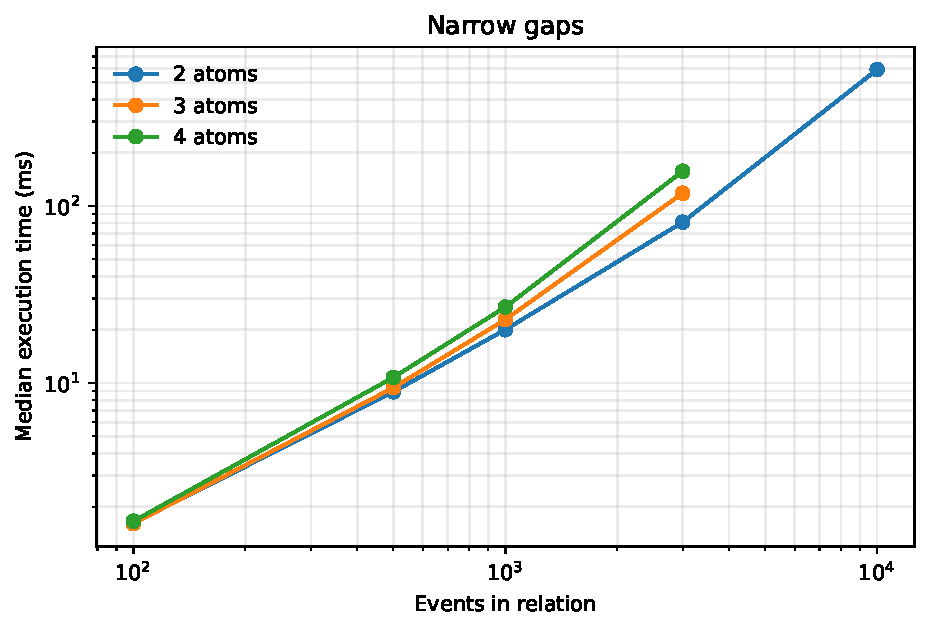
\includegraphics[width=\textwidth]{figures/compiler_microbenchmark_narrow_en.pdf}
\caption{Narrow gaps.}
\end{subfigure}
\hfill
\begin{subfigure}{0.48\textwidth}
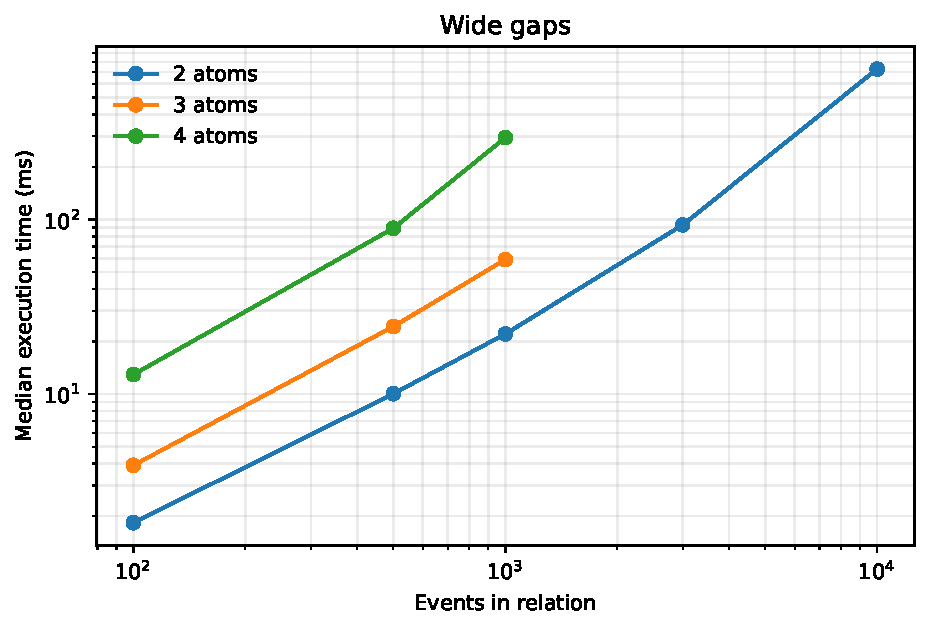
\includegraphics[width=\textwidth]{figures/compiler_microbenchmark_wide_en.pdf}
\caption{Wide gaps.}
\end{subfigure}
\caption{Scaling behavior of the temporal-join plan.}
\label{fig:microbenchmark}
\end{figure}

\section{Synthetic Benchmark of Extraction Pipelines}

\subsection{Corpus, Split, and Patterns}

Six hundred daily series of 365 points are generated with seeds $91000,\ldots,91599$. The first 180 are used exclusively to calibrate one threshold per pipeline and query; the remaining 420 form an evaluation split separate from calibration. Noise levels $\sigma\in\{6,12,20\}$ are balanced.

Each series combines a level $U(160,260)$, a slope $U(-0.05,0.08)$, a weekly sawtooth
\begin{equation}
 [-42,-24,-10,4,24,52,-6]\times U(0.7,1.3),
\end{equation}
an annual sinusoid with amplitude $U(4,18)$, a beginning- and end-of-month effect $U(5,15)$, and AR(1) noise with coefficient $U(0.15,0.45)$. Each pattern family is selected with probability $0.38$, with local exclusion to reduce overlap. Amplitudes lie in $U(45,95)$, and boundaries may be triangular or trapezoidal.

\begin{figure}[H]
\centering
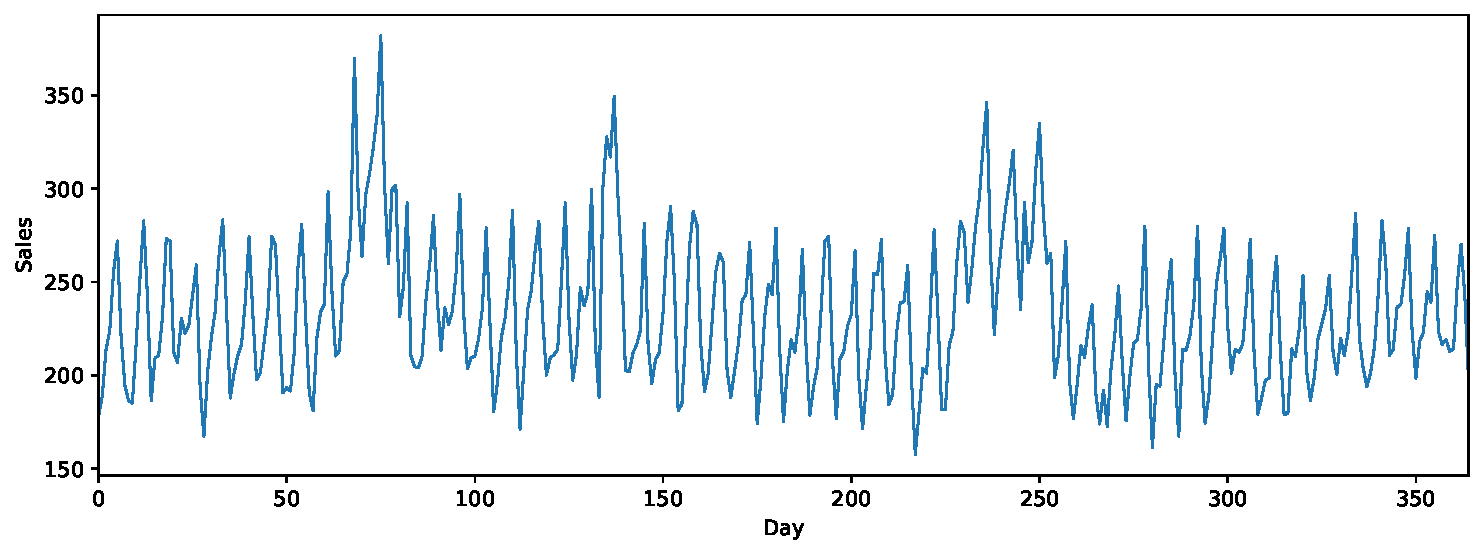
\includegraphics[width=0.96\textwidth]{figures/representative_retail_series_en.pdf}
\caption{Representative synthetic retail-like series with a weekly sawtooth, slow components, autocorrelated noise, and injected transitions.}
\label{fig:retail-example}
\end{figure}

\begin{table}[H]
\centering
\caption{Evaluated morphological queries.}
\label{tab:queries}
\small
\begin{tabularx}{\textwidth}{@{}p{1.1cm}p{5.2cm}X@{}}
\toprule
ID & Expression & Description \\
\midrule
Q1 & $+\xrightarrow{1\text{--}4\,\mathrm{d}}-$ & brief peak \\
Q2 & $+\xrightarrow{8\text{--}14\,\mathrm{d}}-$ & bounded positive episode \\
Q3 & $+\xrightarrow{18\text{--}28\,\mathrm{d}}-$ & long positive episode \\
Q4 & $-\xrightarrow{5\text{--}10\,\mathrm{d}}+$ & temporary trough \\
Q5 & $+\xrightarrow{8\text{--}14\,\mathrm{d}}-\xrightarrow{5\text{--}10\,\mathrm{d}}+$ & rise, fall, rebound \\
Q6 & $+\xrightarrow{1\text{--}4\,\mathrm{d}}-\xrightarrow{3\text{--}10\,\mathrm{d}}+\xrightarrow{1\text{--}4\,\mathrm{d}}-$ & two nearby peaks \\
\bottomrule
\end{tabularx}
\end{table}

\subsection{Comparison, Calibration, and Matching}

The four pipelines share preprocessing, queries, engine, and evaluation protocol, but differ in their extraction rules. The comparison is therefore between complete pipelines. For each pipeline--query pair, a threshold is selected on the calibration split from 100 quantiles constructed from \emph{all} candidate scores. The criterion is F1, with precision and then recall as tie-breakers. Deduplication uses an $L_\infty$ tolerance of two days before calibration and evaluation and is serialized in the protocol.

A prediction and a ground-truth instance of equal length are compatible when their $L_\infty$ distance is at most three days. Optimal bipartite matching first maximizes the number of compatible pairs and then minimizes total boundary error. The 95\% intervals are based on 2,000 paired bootstrap replicates at the series level within the evaluation split, using seed 20260805. They quantify evaluation uncertainty \emph{conditional} on the calibration split and the resulting thresholds; they do not propagate the variability of drawing a new calibration split. Pairwise contrasts are exploratory and not adjusted for multiplicity.

\subsection{Artifact Lineage}

The distributed candidate tables, extraction configurations, and implementation fingerprints are treated as immutable source artifacts. Metric computation, bootstrap intervals, and output manifests are recorded separately from candidate generation. The language and witness contract does not change the extractors, candidate scores, or benchmark labels. The artifact manifest records whether raw candidate generation was rerun and identifies the exact implementation and configuration fingerprints used at each stage.

\subsection{Global Results}

\begin{figure}[H]
\centering
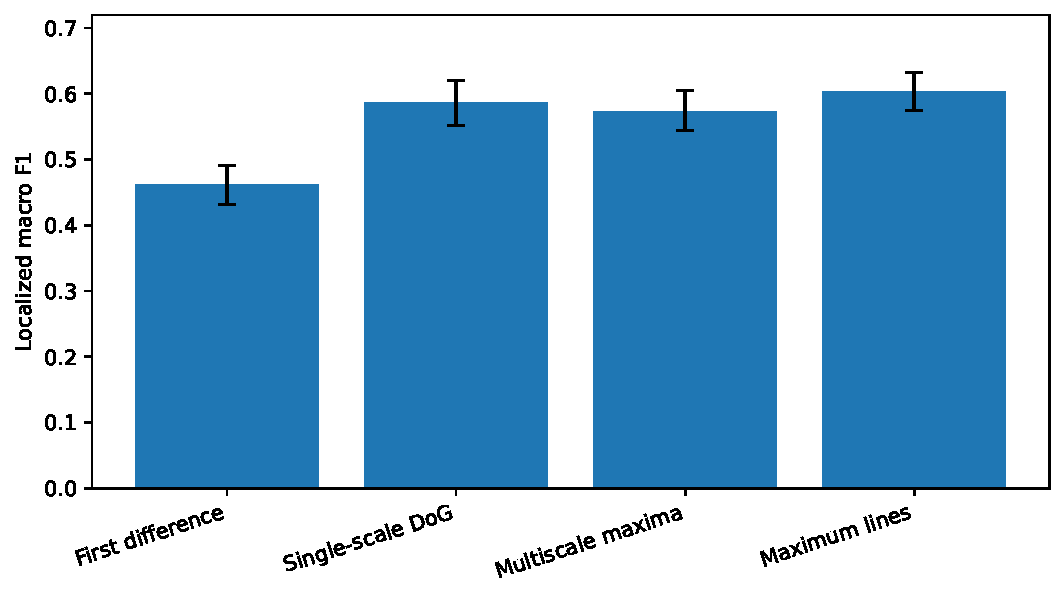
\includegraphics[width=0.82\textwidth]{figures/f1_macro_methods_en.pdf}
\caption{Localized macro F1 on the 420-series evaluation split. The 95\% bootstrap intervals are conditional on fixed calibration.}
\label{fig:global-f1}
\end{figure}

\begin{table}[H]
\centering
\caption{Global pipeline performance. Extraction runtimes come from the archived reference run and are reported descriptively; they are not included in statistical comparisons.}
\label{tab:global-results}
\scriptsize
\begin{tabular*}{\textwidth}{@{\extracolsep{\fill}}lrrrrrr@{}}
\toprule
Pipeline & Macro P & Macro R & Macro F1 [CI] & Micro F1 [CI] & events/series & ms/series \\
\midrule
First difference & .527 & .434 & .462 [.431;.491] & .489 [.458;.518] & 107.0 & 3.468 \\
Single-scale DoG & .735 & .491 & .587 [.552;.620] & .604 [.573;.635] & 46.4 & 1.857 \\
Multiscale maxima & .746 & .475 & .573 [.544;.604] & .592 [.564;.620] & 46.1 & 6.804 \\
Maximum lines & .768 & .503 & \textbf{.604} [.575;.632] & \textbf{.627} [.600;.654] & 49.9 & 12.084 \\
\bottomrule
\end{tabular*}
\end{table}

The runtime environment and provenance are distributed with the reference artifacts. The values locate the computational cost of the prototype; they do not support a statistical performance comparison or characterize a production database system.

On this split, all three wavelet pipelines have higher point estimates than first differences. The paired macro-F1 gain is $+0.125$ for single-scale DoG, $+0.112$ for aggregated maxima, and $+0.142$ for maximum lines; the conditional intervals exclude zero. Maximum lines have the highest global point estimate. Their gain over DoG is $+0.017$, with 95\% CI $[-0.006,0.040]$, so a global advantage is not established. The maximum-lines versus aggregated-maxima contrast is $+0.030$, CI $[0.012,0.049]$, on this split, but it is exploratory, unadjusted, and its point ordering reverses in the additional-seed replication. It does not support a general dominance claim.

\begin{figure}[H]
\centering
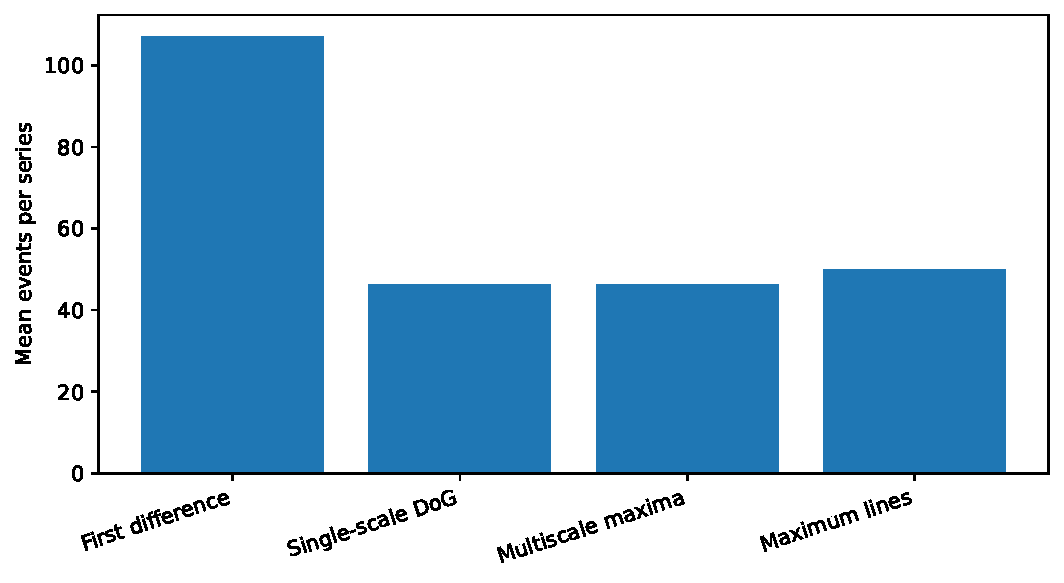
\includegraphics[width=0.76\textwidth]{figures/event_count_methods_en.pdf}
\caption{Mean number of materialized events per series before query execution.}
\label{fig:event-count}
\end{figure}

\subsection{Results by Query and Noise Level}

\begin{figure}[H]
\centering
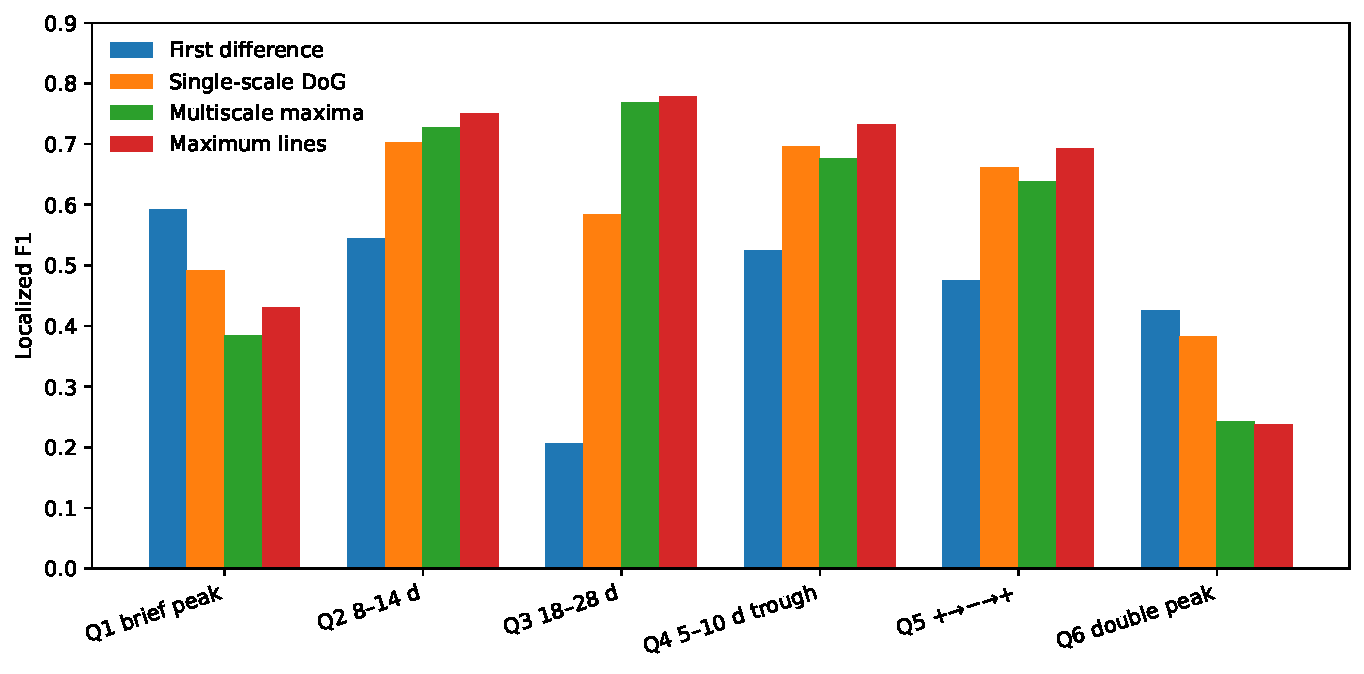
\includegraphics[width=0.98\textwidth]{figures/f1_by_query_en.pdf}
\caption{Localized F1 by query and pipeline.}
\label{fig:query-f1}
\end{figure}

\begin{table}[H]
\centering
\caption{F1 by query family.}
\small
\begin{tabular}{lrrrr}
\toprule
Query & First diff. & Single DoG & Multi. maxima & Max. lines \\
\midrule
Q1 brief peak & \textbf{.592} & .492 & .384 & .430 \\
Q2 8--14 d episode & .544 & .703 & .728 & \textbf{.751} \\
Q3 18--28 d episode & .207 & .584 & .769 & \textbf{.779} \\
Q4 5--10 d trough & .525 & .696 & .677 & \textbf{.733} \\
Q5 $+\!\to\!-\!\to\!+$ & .475 & .661 & .639 & \textbf{.693} \\
Q6 double peak & \textbf{.426} & .383 & .243 & .237 \\
\bottomrule
\end{tabular}
\end{table}

Maximum lines are useful for persistent episodes and Q5. They are unfavorable for brief peaks, whose boundaries merge or disappear when cross-scale persistence is required. A practical policy should select a fine branch for Q1/Q6 and a multiscale branch for more persistent structures; this hybrid policy is not evaluated here.

\begin{figure}[H]
\centering
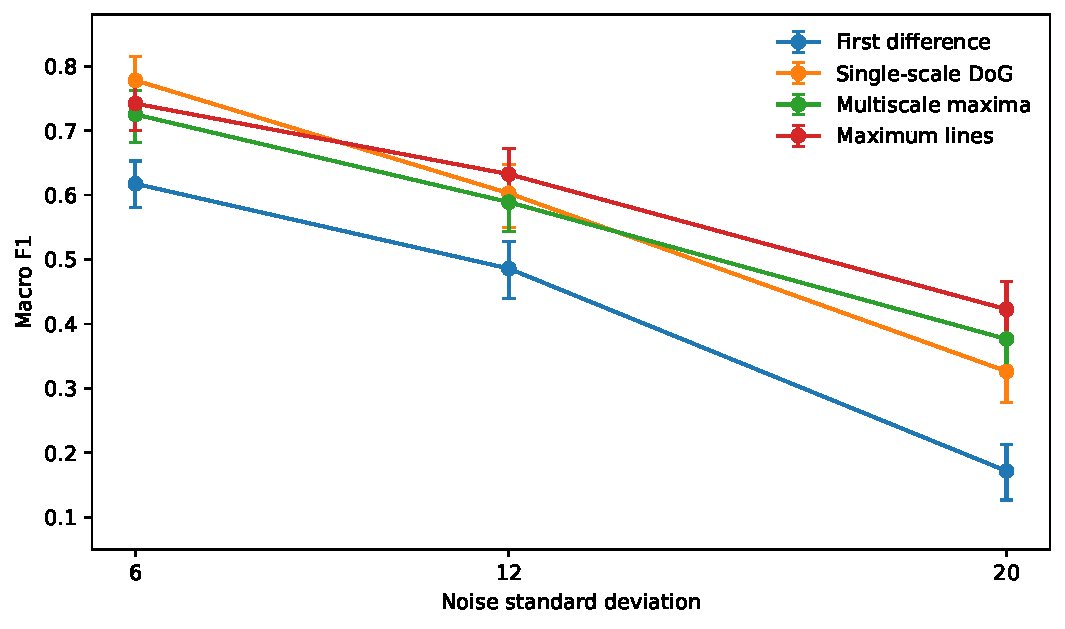
\includegraphics[width=0.82\textwidth]{figures/f1_by_noise_en.pdf}
\caption{Macro F1 by noise level, with bootstrap intervals.}
\label{fig:noise-f1}
\end{figure}

At $\sigma=6$, single-scale DoG reaches .778, ahead of maximum lines (.742). At $\sigma=12$, maximum lines reach .632, ahead of DoG (.603). At $\sigma=20$, they reach .423, compared with .326 for DoG and .172 for first differences. Cross-scale persistence becomes useful when local extrema are unstable, but remains costly for short events.

\subsection{Targeted Ablation of the Maximum-Line Pipeline}

A separate experiment uses 300 new series: 90 for calibration and 210 for evaluation. Each variant is calibrated independently on all its candidates. Intervals are based on 2,000 paired bootstrap replicates at the ablation-series level, seed 20260806, conditional on that calibration. They are exploratory and unadjusted for the fifteen pairwise contrasts among variants.

\begin{figure}[H]
\centering
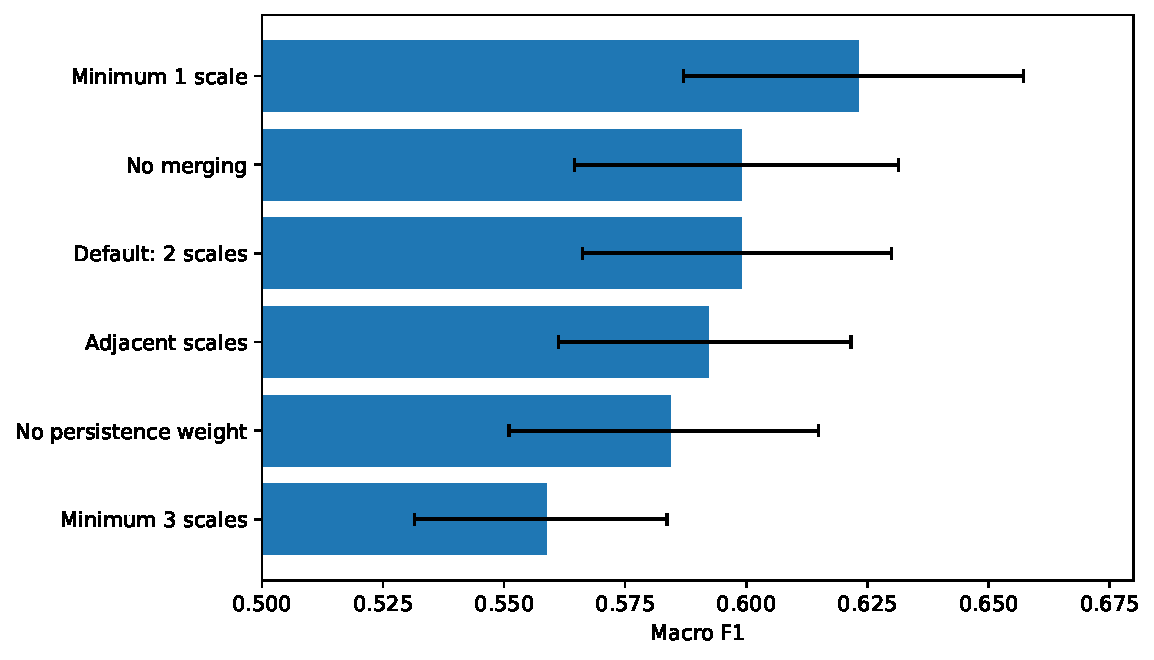
\includegraphics[width=0.88\textwidth]{figures/wtmm_ablation_en.pdf}
\caption{Macro F1 of maximum-line extractor variants on the ablation corpus.}
\label{fig:ablation}
\end{figure}

\begin{table}[H]
\centering
\caption{Targeted ablation with paired bootstrap intervals.}
\small
\begin{tabularx}{\textwidth}{@{}Xrrrr@{}}
\toprule
Variant & Macro P & Macro R & Macro F1 [95\% CI] & events/series \\
\midrule
Minimum 1 scale & .686 & .589 & \textbf{.623} [.587;.657] & 89.1 \\
No merging & .765 & .518 & .599 [.565;.631] & 50.7 \\
Default, minimum 2 scales & .713 & .528 & .599 [.566;.630] & 50.0 \\
Strictly adjacent scales & .701 & .523 & .592 [.561;.622] & 49.7 \\
No persistence weighting & .681 & .530 & .584 [.551;.615] & 50.0 \\
Minimum 3 scales & .681 & .483 & .559 [.532;.584] & 33.8 \\
\bottomrule
\end{tabularx}
\end{table}

Allowing a single scale increases F1 by $0.024$ relative to the default, with paired interval $[0.0003,0.048]$, but raises the relation from 50 to 89 events per series and abandons the strong notion of cross-scale persistence. Requiring three scales decreases F1 by $0.040$, interval $[-0.062,-0.018]$, and produces a sparser relation. Disabling merging is close to the default in this experiment ($\Delta=0.00025$, interval $[-0.0076,0.0076]$). These intervals are exploratory and unadjusted for the fifteen multiple comparisons among six variants. They establish neither optimality nor general superiority; the robust result is the trade-off among recall, relational cardinality, and auditability. The ablation is partial: it does not cover preprocessing, multiple scale grids, or a complete nested hyperparameter selection.

\subsection{Replication on Additional Seeds}

With code, hyperparameters, split sizes, and calibration procedure fixed, an additional corpus of 120 series is generated from seeds $130000,\ldots,130119$. The thresholds are not reused from the main benchmark: they are recalibrated under the fixed procedure on 40 new series and evaluated on 80 new series. This is a qualitative replication of the complete procedure under additional seeds, not an application of the original thresholds and not an independent preregistration. Its size does not justify a definitive ranking or new inferential claims.

\begin{table}[H]
\centering
\caption{Replication on 80 additional evaluation series.}
\label{tab:additional_seed}
\small
\begin{tabular}{lrrr}
\toprule
Pipeline & Macro precision & Macro recall & Macro F1 \\
\midrule
First difference & .496 & .513 & .477 \\
Single-scale DoG & .898 & .521 & .641 \\
Multiscale maxima & .842 & .607 & \textbf{.691} \\
Maximum lines & .811 & .621 & .679 \\
\bottomrule
\end{tabular}
\end{table}

The point estimates of all three wavelet branches remain above first differences, but aggregated maxima exceed maximum lines on this split. This reversal confirms that the best representation depends on the corpus. Maximum lines provide explicit cross-scale persistence and coefficient-level provenance. Their event cardinality is comparable to that of the other wavelet pipelines and varies with the persistence criterion, so sparsity should be understood as a tunable trade-off rather than an unconditional advantage.

\section{Exploratory Observational Study on Real Sales}

\subsection{Data and Protocol}

The pipeline is applied retrospectively to five daily product--store series from January 2, 2023, to June 7, 2026, corresponding to 1,253 days and 6,265 observations in total. Coverage ranges from 96.6\% to 98.9\%; missing dates are set to zero under the available historical protocol. Table~\ref{tab:real-series} describes the sample under systematic anonymization, while repeated products and sites are retained to preserve the sample structure.

\begin{table}[H]
\centering
\caption{Series included in the observational study.}
\label{tab:real-series}
\small
\begin{tabularx}{\textwidth}{@{}lXlrr@{}}
\toprule
ID & Product & Store & Coverage & Zeros \\
\midrule
S1 & Product A (250 g format) & Site 1 & 98.9\% & 1.1\% \\
S2 & Product A (250 g format) & Site 2 & 98.4\% & 1.6\% \\
S3 & Product B (250 g format) & Site 1 & 96.6\% & 3.4\% \\
S4 & Product A (250 g format) & Site 3 & 96.6\% & 3.4\% \\
S5 & Product B (250 g format) & Site 4 & 96.7\% & 3.3\% \\
\bottomrule
\end{tabularx}
\end{table}

The same centered 63-day preprocessing is used; the analysis is therefore descriptive and non-causal. Three queries are executed: Q1 (1--4 days), Q2 (8--14 days), and Q3 (18--28 days), with fixed score thresholds 1.358377, 1.409728, and 1.403736, respectively. Prices and promotional markers, available only incompletely, are joined \emph{after} retrieval for exploratory description.

\subsection{Descriptive Results}

Forty-four matches are obtained and consolidated into 28 unique temporal episodes. Table~\ref{tab:real-results} reports the aggregate results. Detected lift is the ratio of sales within a retrieved window to a local reference level; control lift comes from matched control windows under the internal protocol. The distributed artifacts provide the input schema, a generic aggregation script, de-identified aggregates, and a processing manifest. Proprietary data and row-level annotations are not redistributed. The observational analysis is therefore only partially reproducible rather than fully replayable by a third party.

\begin{table}[H]
\centering
\caption{Observational aggregates. ``Median promo'' is the median across series of the fraction of marked units within windows; it is not the fraction of episodes containing at least one marker.}
\label{tab:real-results}
\small
\begin{tabular}{lrrrrrr}
\toprule
Query & Matches & Series & Detected lift & Control lift & Excess & Median promo \\
\midrule
Q1 (1--4 d) & 13 & 5 & 1.564 & .943 & +.737 & 0.0\% \\
Q2 (8--14 d) & 19 & 5 & 1.402 & .997 & +.405 & 85.5\% \\
Q3 (18--28 d) & 12 & 4 & 1.004 & .982 & +.037 & 6.7\% \\
Unique episodes & 28 & 5 & 1.392 & .984 & +.383 & 0.0\% \\
\bottomrule
\end{tabular}
\end{table}

Among the three series with usable annotations, 18 episodes can be compared with the markers: 7 contain at least one marked unit and 11 contain none. This count is not inconsistent with the zero median for unique episodes because the denominators and aggregation procedures differ. The aggregate median price change is close to zero; the positive $+0.004$ point in the global row is a change in a ratio and does not demonstrate a price reduction.

The windows are selected precisely because they contain salient sales shapes, so a high sales lift is partly tautological. The concentration of markers in Q2 is a descriptive signal compatible with some intermediate-duration episodes, but the sample size, incomplete labels, and dependence among observations preclude characterizing MorphoQL as a general promotion detector.

\subsection{Stability and Drift}

With thresholds fixed, the observed detection rate increases from approximately 1.05 to 1.71 episodes per series--year--query, a ratio of 1.63; Q2 reaches about 2.22. A second extraction branch corroborates approximately 50\% of episodes under the selected agreement window. These values indicate drift in score or event frequency, but corroboration is not independent because the methods share the signal and part of the preprocessing. A production system should monitor this drift and recalibrate using past-only windows.

\subsection{Scope of the Study}

The study establishes that the pipeline can operate without injected patterns and produce interpretable witnesses. It provides neither blindly annotated morphological ground truth, nor a sufficiently large sample, nor causal control. It therefore cannot estimate real query accuracy or attribute episodes to a commercial intervention.

\section{Discussion}

\subsection{What MorphoQL Contributes}

The main contribution is an explicit interface among four layers:
\begin{equation}
\begin{aligned}
 \text{signal and coefficients}
 &\longrightarrow \text{multi-series event relation}\\
 &\longrightarrow \text{morphological program}
 \longrightarrow \text{execution witness}.
\end{aligned}
\end{equation}
The language does not depend on the complete coefficient matrix; it depends on an event contract. The relation can be indexed, joined with metadata, and audited. The program can be validated independently of the extractor, while the witness reconnects a match to numerical nodes without conflating traceability with causal truth.

\subsection{What the Validation Establishes and Does Not Establish}

The 800 differential cases without mismatch support consistency among three execution strategies on the tested core. They prove neither the absence of every software defect, nor extractor fidelity, nor completeness of a broader language. Likewise, the microbenchmark characterizes a direct Python implementation on relations of up to 10,000 events; it does not establish database scalability or competitiveness with a CEP engine.

\subsection{Why Maximum Lines Should Not Be the Only Branch}

Maximum lines suppress unstable maxima and expose persistence. The benchmark confirms their usefulness under noise and for episodes lasting several weeks. However, this selection removes part of the information carried by brief peaks. The ablation reinforces this diagnosis: reducing the persistence requirement to one scale increases F1 but nearly doubles the number of events. A morphological planner should therefore trade off a fine branch, a multiscale branch, and expected relational cost. Such a policy remains to be evaluated.

\subsection{Natural Language and Vector Retrieval}

A language model can translate a free-form request into Core 0.2 and allow the parser to validate the resulting program. The decision remains symbolic and auditable. For vague queries not expressible by the core, a maximum-line encoder could produce a compact vector aligned with a pretrained text encoder. A natural hybrid architecture uses hard constraints in MorphoQL and residual similarity in a latent space. This extension is not implemented or evaluated here.

\subsection{Morphological Rewriting and Counterfactuals}

An explicit query supports controlled rewriting, for example replacing $[8,14]$ with $[18,28]$ or reversing a sign. Retrieving observed episodes satisfying the rewritten expression provides morphological analogues. This is shape editing or a morphological counterfactual, not a causal counterfactual for sales.

\section{Limitations and Threats to Validity}

\begin{enumerate}
  \item \textbf{Narrow core.} Only \code{EDGE--THEN--WITHIN} chains are normative. Interval, oscillatory, and Boolean primitives remain future work.
  \item \textbf{Relative correctness.} Equivalence concerns an already extracted finite relation; it does not prove that the events capture every relevant transition in the signal.
  \item \textbf{Heuristic extractors.} Thresholds, link costs, strength rules, and merging rules are hand-designed. The ablation is targeted rather than a complete nested hyperparameter selection.
  \item \textbf{Heuristic score.} Score coefficients are not derived from a probabilistic theory; they support ranking and calibration.
  \item \textbf{Retrospective preprocessing.} The centered median and global weekly profile introduce temporal leakage if the experiment is interpreted as streaming.
  \item \textbf{Pipeline comparison.} Branches have pipeline-specific hyperparameters and event densities. The benchmark does not isolate the causal effect of multiscale analysis or linking.
  \item \textbf{Conditional uncertainty.} Main-benchmark intervals condition on the calibration split and thresholds; pairwise contrasts are exploratory and unadjusted for multiplicity.
  \item \textbf{Synthetic data.} Injected patterns have controlled boundaries and do not cover all irregular sampling, missingness, intermittent demand, or real retail frequencies.
  \item \textbf{Incomplete baselines.} The evaluation lacks detection comparisons with segmentation, shape expressions, STL/SSTS/T-ReX, the Matrix Profile, and learned models under common annotations.
  \item \textbf{Witness scope.} Recomputation establishes consistency relative to the relation, implementation, and bound policy; it does not guarantee authenticity of an unanchored policy or identify the producer.
  \item \textbf{Interoperable canonicalization.} Fingerprints use a deterministic JSON serialization defined by the Python prototype. Cross-language verification requires an independent specification of numbers, Unicode, key ordering, and composite values.
  \item \textbf{Limited microbenchmark.} Peak memory, index optimization, and comparison with an industrial engine are not reported. At 10,000 events, only two-atom plans are measured.
  \item \textbf{Small real-data study.} Five product--store series provide neither independent morphological ground truth, adequate statistical power, nor causal validation.
  \item \textbf{Partial reproducibility of real data.} Proprietary sales and annotations are not redistributed. The schema, generic script, processing steps, and de-identified aggregates are provided, but the private inputs are unavailable.
\end{enumerate}

\section{Conclusion}

MorphoQL Core 0.2 demonstrates that an event relation derived from time--scale representations can serve as the substrate of a declarative shape-query kernel. Relation-bound verification recompiles a program, recomputes the strict set, reproduces ordering, deduplication, and limit, rematerializes every projected row, and compares column order, values, and the fingerprint of the complete projected output. The nested AST schema and programmatic API enforce a strict type system without silent coercion.

The validation accepts 1,200 unique positive queries, rejects 1,200 derived invalid mutations, passes 85 adversarial cases, and observes no mismatch across 800 differential cases comparing enumeration, Python joins, and SQLite. These tests support the implementation of the evaluated core without replacing a general proof of software correctness, a cryptographic signature of the witness, or validation of extractor fidelity.

On the main synthetic generator, the three wavelet pipelines have point estimates above first differences. Maximum lines achieve the highest global point estimate and are more robust under high noise, but their advantage over single-scale DoG is not established at the 95\% level. Main intervals condition on fixed calibration, and pairwise contrasts are not adjusted for multiplicity. The additional-seed replication recalibrates thresholds under the fixed procedure and reverses the point ordering between aggregated maxima and maximum lines. These results motivate a hybrid planner rather than exclusive use of one representation.

The observational study establishes retrospective feasibility, not general morphological accuracy or a promotional or causal interpretation. The next steps are blindly annotated ground truth over a larger collection of real series, causal preprocessing for streaming use, stronger language and detection baselines, relational optimization, and normative extension of the language one primitive at a time.

\appendix

\section{Maximum-Line Linking Pseudocode}

\begin{lstlisting}[language={},basicstyle=\ttfamily\footnotesize]
for sign in {+1, -1}:
    active = []
    finished = []
    for scale_index, scale in increasing_scales:
        nodes = maxima[scale_index, sign]
        candidate_links = []
        for line in active:
            if scale_index - line.last_scale_index <= max_scale_skip:
                tolerance = max(2, 0.65 * scale + 1)
                for node in nodes:
                    if abs(node.time - line.last_time) <= tolerance:
                        cost = abs(node.time-line.last_time)/tolerance
                               - 0.03 * node.strength
                        candidate_links.append((cost, line, node))
        greedily assign links by increasing cost
        finish lines absent for more than max_scale_skip indices
        start one line for each unassigned node
    keep lines covering at least min_scales distinct scales
    compute representative time, persistence, strength,
        scale span, and ordered supporting nodes
merge same-sign lines separated by at most merge_days
    while preserving the union of all supporting nodes
assign content-addressed (series_id, event_id)
emit events above the event threshold
\end{lstlisting}

\section{Reproducibility and Artifacts}

The accompanying artifact provides source code, tests, registered configurations, reference outputs, figures, and the \LaTeX{} source. Correctness validation and load testing are separated:
\begin{lstlisting}[language={},basicstyle=\ttfamily\footnotesize]
./run_validation_fast.sh
./run_microbenchmark.sh
./run_full_benchmark.sh
PYTHONPATH=src python src/verify_results_v8.py
./build_paper_english.sh
\end{lstlisting}
By default, scripts write to reproduction directories and do not modify reference outputs. Setting \code{MORPHOQL\_OVERWRITE\_REFERENCE=1} enables intentional refresh. The \path{src/configuration.py} registry generates the configuration JSON files and is the common source for extraction, witnesses, and the experimental protocol.

\begin{table}[H]
\centering
\caption{Compliance table for the main reproducible claims.}
\scriptsize
\begin{tabularx}{\textwidth}{@{}p{3.0cm}X X@{}}
\toprule
Claim & Artifact and command & Expected output \\
\midrule
Fast validation & \path{tests/validate_core_v02.py}; \path{./run_validation_fast.sh} & 1,200 positive, 1,200 negative, 85/85 adversarial cases \\
Differential equivalence & same script & 800 cases, 0 mismatches across three engines \\
Provenance and witness & \path{results/execution_witness_example_v8.json}; \path{results/execution_witness_verification_v8.json} & occurrence and SELECT rows reproduced; projector, value, and manifest tampering rejected \\
Microbenchmark & \path{tests/run_microbenchmark_v7.py}; \path{results/compiler_microbenchmark_protocol_v7.json} & exact matrix of executed cells up to 10,000 events \\
Benchmark and bootstrap & \path{src/benchmark_morphoql_v7.py}, \path{src/postprocess_v7.py} & all calibration candidates, 2,000 replicates \\
Paired ablation & \path{src/ablation_wtmm_v7.py} & six variants; exploratory unadjusted intervals \\
Additional-seed replication & \path{src/additional_seed_replication_v7.py} & 40 new calibration series, 80 evaluation series; thresholds recalibrated under the fixed procedure \\
Numerical verification & \path{src/verify_results_v8.py} & invariants and numerical results within tolerances, excluding runtimes \\
English figures & \path{src/make_figures_english.py} & English PDF and PNG figures \\
\bottomrule
\end{tabularx}
\end{table}

Checksums distinguish inputs, code, and reference outputs. The implementation fingerprint included in each witness is computed over the engine and configuration registry; relation and manifest fingerprints identify the event input and ordered outputs. \code{verify\_witness} checks these claims by recomputation when the required objects are supplied. This does not prove prior existence or the identity of the witness producer. Execution times are not compared through exact equality. For the observational study, the artifacts provide the schema, generic script, and anonymized aggregates, but not proprietary inputs.

\section{Complete Maximum-Line Results}

\begin{table}[H]
\centering
\small
\caption{Maximum-line results on the 420-series evaluation split.}
\begin{tabular}{lrrrrr}
\toprule
Query & TP & FP & FN & Precision & Recall / F1 \\
\midrule
Q1 & 157 & 92 & 324 & .631 & .326 / .430 \\
Q2 & 266 & 20 & 156 & .930 & .630 / .751 \\
Q3 & 118 & 17 & 50 & .874 & .702 / .779 \\
Q4 & 290 & 42 & 169 & .873 & .632 / .733 \\
Q5 & 80 & 8 & 63 & .909 & .559 / .693 \\
Q6 & 27 & 42 & 132 & .391 & .170 / .237 \\
\bottomrule
\end{tabular}
\end{table}

\begin{thebibliography}{99}

\bibitem{agrawal1995}
R. Agrawal, G. Psaila, E. L. Wimmers, and M. Za\"it.
\newblock Querying shapes of histories.
\newblock In \emph{Proceedings of the 21st International Conference on Very Large Data Bases (VLDB)}, pages 502--514, 1995.

\bibitem{allen1983}
J. F. Allen.
\newblock Maintaining knowledge about temporal intervals.
\newblock \emph{Communications of the ACM}, 26(11):832--843, 1983.

\bibitem{faloutsos1994}
C. Faloutsos, M. Ranganathan, and Y. Manolopoulos.
\newblock Fast subsequence matching in time-series databases.
\newblock In \emph{Proceedings of ACM SIGMOD}, pages 419--429, 1994.

\bibitem{mallat1992}
S. Mallat and W. L. Hwang.
\newblock Singularity detection and processing with wavelets.
\newblock \emph{IEEE Transactions on Information Theory}, 38(2):617--643, 1992.

\bibitem{hochheiser2004}
H. Hochheiser and B. Shneiderman.
\newblock Dynamic query tools for time series data sets: Timebox widgets for interactive exploration.
\newblock \emph{Information Visualization}, 3(1):1--18, 2004. doi:10.1057/palgrave.ivs.9500061.

\bibitem{maler2004}
O. Maler and D. Ni\v{c}kovi\'c.
\newblock Monitoring temporal properties of continuous signals.
\newblock In \emph{FORMATS/FTRTFT}, pages 152--166, 2004. doi:10.1007/978-3-540-30206-3\_12.

\bibitem{donze2010}
A. Donz\'e and O. Maler.
\newblock Robust satisfaction of temporal logic over real-valued signals.
\newblock In \emph{FORMATS}, pages 92--106, 2010. doi:10.1007/978-3-642-15297-9\_9.

\bibitem{gyllstrom2007}
D. Gyllstrom, E. Wu, H.-J. Chae, Y. Diao, P. Stahlberg, and G. Anderson.
\newblock SASE: Complex event processing over streams.
\newblock In \emph{CIDR}, 2007.

\bibitem{lin2007}
J. Lin, E. Keogh, L. Wei, and S. Lonardi.
\newblock Experiencing SAX: a novel symbolic representation of time series.
\newblock \emph{Data Mining and Knowledge Discovery}, 15:107--144, 2007.

\bibitem{nickovic2018}
D. Ni\v{c}kovi\'c, O. Lebeltel, O. Maler, T. Ferr\`ere, and D. Ulus.
\newblock AMT 2.0: Qualitative and quantitative trace analysis with extended Signal Temporal Logic.
\newblock In \emph{TACAS}, pages 303--319, 2018. doi:10.1007/978-3-319-89963-3\_18.

\bibitem{rodrigues2019}
J. Rodrigues, D. Folgado, D. Belo, and H. Gamboa.
\newblock SSTS: A syntactic tool for pattern search on time series.
\newblock \emph{Information Processing \& Management}, 56(1):61--76, 2019. doi:10.1016/j.ipm.2018.09.001.

\bibitem{mamouras2017}
K. Mamouras, M. Raghothaman, R. Alur, Z. G. Ives, and S. Khanna.
\newblock StreamQRE: Modular specification and efficient evaluation of quantitative queries over streaming data.
\newblock In \emph{Proceedings of PLDI}, pages 693--708, 2017. doi:10.1145/3062341.3062369.

\bibitem{abbas2019}
H. Abbas, A. Rodionova, E. Bartocci, S. A. Smolka, and R. Grosu.
\newblock Quantitative regular expressions for arrhythmia detection algorithms.
\newblock \emph{IEEE/ACM Transactions on Computational Biology and Bioinformatics}, 16(5):1586--1597, 2019. doi:10.1109/TCBB.2018.2885274.

\bibitem{kong2020}
L. Kong and K. Mamouras.
\newblock StreamQL: A query language for processing streaming time series.
\newblock \emph{Proceedings of the ACM on Programming Languages}, 4(OOPSLA), Article 183, 2020. doi:10.1145/3428251.

\bibitem{siddiqui2020}
T. Siddiqui, P. Luh, Z. Wang, K. Karahalios, and A. Parameswaran.
\newblock ShapeSearch: A Flexible and Efficient System for Shape-based Exploration of Trendlines.
\newblock In \emph{Proceedings of the 2020 ACM SIGMOD International Conference on Management of Data}, pages 51--65, 2020. doi:10.1145/3318464.3389722.

\bibitem{yu2023}
Y. Yu, T. Becker, L. M. Trinh, and M. Behrisch.
\newblock SAXRegEx: Multivariate time series pattern search with symbolic representation, regular expression, and query expansion.
\newblock \emph{Computers \& Graphics}, 112:13--21, 2023. doi:10.1016/j.cag.2023.03.002.

\bibitem{nickovic2021}
D. Ni\v{c}kovi\'c, X. Qin, T. Ferr\`ere, C. Mateis, and J. Deshmukh.
\newblock Specifying and detecting temporal patterns with shape expressions.
\newblock \emph{International Journal on Software Tools for Technology Transfer}, 23:565--577, 2021. doi:10.1007/s10009-021-00627-x.

\bibitem{petkovic2022}
D. Petkovi\'c.
\newblock Specification of row pattern recognition in the SQL standard and its implementations.
\newblock \emph{Datenbank-Spektrum}, 22:163--174, 2022.

\bibitem{zhu2023}
E. Zhu, S. Huang, and S. Chaudhuri.
\newblock High-performance row pattern recognition using joins.
\newblock \emph{Proceedings of the VLDB Endowment}, 16(5):1181--1194, 2023. doi:10.14778/3579075.3579090.

\bibitem{huang2023}
S. Huang, E. Zhu, S. Chaudhuri, and L. Spiegelberg.
\newblock T-ReX: Optimizing pattern search on time series.
\newblock In \emph{Proceedings of ACM SIGMOD}, 2023. doi:10.1145/3589275.

\bibitem{lilly2010}
J. M. Lilly and S. C. Olhede.
\newblock On the analytic wavelet transform.
\newblock \emph{IEEE Transactions on Information Theory}, 56(8):4135--4156, 2010.

\bibitem{lilly2017}
J. M. Lilly.
\newblock Element analysis: a wavelet-based method for analysing time-localized events in noisy time series.
\newblock \emph{Proceedings of the Royal Society A}, 473:20160776, 2017.

\bibitem{yeh2016}
C.-C. M. Yeh et al.
\newblock Matrix Profile I: All pairs similarity joins for time series.
\newblock In \emph{IEEE ICDM}, pages 1317--1322, 2016.

\bibitem{ito2024}
A. Ito, K. Dohi, and Y. Kawaguchi.
\newblock CLaSP: Learning concepts for time-series signals from natural language supervision.
\newblock arXiv:2411.08397, 2024; revised 2025.

\bibitem{chen2025}
Z. Chen, X. Zhang, and M. Zhu.
\newblock TS-CLIP: Time Series Understanding by CLIP.
\newblock In \emph{Proceedings of EMNLP}, pages 4646--4664, 2025.

\bibitem{tan2026}
Z. Tan, Y. Zhao, S. Wang, C. Xu, Y. Liang, X. Liu, S. Pan, and M. Jin.
\newblock Sonar-TS: Search-Then-Verify Natural Language Querying for Time Series Databases.
\newblock Accepted at \emph{ICML 2026}; arXiv:2602.17001v3, 2026.

\bibitem{dohi2026}
K. Dohi et al.
\newblock LaSTR: Language-driven time-series segment retrieval.
\newblock arXiv:2603.00725, 2026.

\bibitem{wan2026}
S. C. Wan, Y. Y. Wang, T. Hou, X. Chang, and A. Jan.
\newblock Grammar of the Wave: Towards explainable multivariate time series event detection via neuro-symbolic VLM agents.
\newblock arXiv:2603.11479v3, 2026.

\bibitem{kim2026}
J. Kim, C. Oh, S. Lee, I. Rish, and C. Lee.
\newblock Representing Time Series as Structured Programs for LLM Reasoning.
\newblock arXiv:2606.12481v1, 2026.

\bibitem{litsseek2026}
X. Li, K. Alnuaim, M. Y. Eltabakh, and E. A. Rundensteiner.
\newblock TSseek: Regular Expression-Based Similarity Search for Distributed Time Series Datasets.
\newblock arXiv:2606.09824, 2026.

\bibitem{sun2026}
G. Sun, Y. Chen, E. Guo, Y. Yao, and D. Liu.
\newblock ShapeTalk: Combining natural language and sketch for time-series pattern querying.
\newblock arXiv:2607.07073, 2026.

\end{thebibliography}

\end{document}
